% =====================================================================
%  Sections 4--7: Weak solutions, Non-uniqueness, Entropy condition,
%  Riemann problem.
% =====================================================================

\section{Weak Solutions and the Integral Form}
\label{sec:weak-solutions}

Classical solutions of \eqref{eq:ivp} cannot be extended past the breakdown
time $T^*$ of Proposition~\ref{prop:shock-time}, even though nothing in the
underlying physics suggests the evolution should stop. This section weakens
the notion of solution: rather than requiring $u_t+u\,u_x=0$ pointwise, $u$
need only satisfy an integral identity against smooth test functions, which
admits discontinuous solutions for all $t\ge0$; and it derives the condition
such discontinuities must satisfy. The two
verifications needed later --- that a piecewise smooth function is a weak
solution (Proposition~\ref{prop:piecewise-weak}), and what a jump must
satisfy (Theorem~\ref{thm:rankine-hugoniot}) --- are done \emph{once},
here, and reused in Sections~\ref{sec:nonuniqueness} and
\ref{sec:riemann-problem}.

\subsection{The integral formulation}
\label{subsec:integral-form}

Let $u$ be a $C^1$ solution of $u_t + f(u)_x = 0$ on $\mathbb{R} \times
(0,\infty)$ with $f(u)=u^2/2$ and $u(\cdot,0)=u_0$, and let $\varphi \in
C_c^1(\mathbb{R} \times [0,\infty))$ be any test function, compactly
supported but not required to vanish at $t=0$. Multiplying the PDE by
$\varphi$, integrating over $\mathbb{R}\times(0,\infty)$, and integrating
by parts in both $x$ and $t$ (using that $\varphi$ has compact support, so
all boundary terms at spatial infinity vanish) gives
\begin{equation}
  \label{eq:weak-derivation}
  0 = \int_0^\infty\!\!\int_{\mathbb{R}} \big(u_t + f(u)_x\big)\varphi\, dx\, dt
  = -\int_0^\infty\!\!\int_{\mathbb{R}} \big(u\,\varphi_t + f(u)\,\varphi_x\big)\, dx\, dt
  - \int_{\mathbb{R}} u_0(x)\, \varphi(x,0)\, dx,
\end{equation}
where the boundary term at $t=0$ survives because $\varphi(x,0)$ need not
vanish. Equation \eqref{eq:weak-derivation} makes sense whenever $u \in
L^\infty$, with no differentiability required of $u$ at all: this
motivates the following definition.

\begin{definition}[Weak solution]
\label{def:weak-solution}
Let $u_0\in L^\infty(\mathbb{R})$. A function $u \in
L^\infty(\mathbb{R}\times(0,\infty))$ is a \emph{weak solution} of
\eqref{eq:ivp} (with data $u_0$) if
\begin{equation}
  \label{eq:weak-formulation}
  \int_0^\infty\!\!\int_{\mathbb{R}} \big(u\,\varphi_t + f(u)\,\varphi_x\big)\, dx\, dt
  + \int_{\mathbb{R}} u_0(x)\, \varphi(x,0)\, dx = 0
\end{equation}
for every $\varphi \in C_c^1(\mathbb{R}\times[0,\infty))$.
\end{definition}

\noindent\emph{Conventions.} Test functions are always taken in
$C_c^1(\mathbb{R}\times[0,\infty))$. Those that vanish near $t=0$ test only
the PDE in $t>0$; those with $\varphi(\cdot,0)\ne0$ are what impose the
\emph{initial condition}, which enters solely through the term
$\int u_0\varphi(\cdot,0)\,dx$ (an $L^\infty$ function has no pointwise
initial value to speak of).

A $C^1$ function is a weak solution if and only if it is a classical solution:
reading \eqref{eq:weak-derivation} in reverse gives one direction, and for the
other one takes $\varphi$ supported in $t>0$ (forcing $u_t+f(u)_x=0$ pointwise)
and then $\varphi(\cdot,0)$ arbitrary (forcing $u(\cdot,0)=u_0$).

\subsection{Piecewise smooth functions and the Rankine--Hugoniot condition}
\label{subsec:rankine-hugoniot}

All discontinuous solutions in this paper have the following structure.

\begin{definition}[Piecewise $C^1$ function]
\label{def:piecewise}
Let $s_1,\dots,s_k:[0,\infty)\to\mathbb{R}$ be $C^1$ with $s_1(t)<\dots<
s_k(t)$ for $t>0$ (the curves may start at a common point when $t=0$).
Put $s_0\equiv-\infty$, $s_{k+1}\equiv+\infty$ and
$\Omega_i=\{(x,t):\ t>0,\ s_i(t)<x<s_{i+1}(t)\}$ for $i=0,\dots,k$. A
bounded function $u$ is \emph{piecewise $C^1$ with respect to
$s_1,\dots,s_k$} if on each $\Omega_i$ it is $C^1$ and $u,u_x,u_t$ extend
continuously to $\overline{\Omega_i}\cap\{t>0\}$. Along $x=s_i(t)$ we
write $u_\ell(t)$ and $u_r(t)$ for the limits taken from $\Omega_{i-1}$
and $\Omega_i$ respectively.
\end{definition}

\begin{theorem}[Rankine--Hugoniot condition]
\label{thm:rankine-hugoniot}
Let $u$ be piecewise $C^1$ with respect to $s_1,\dots,s_k$, and a weak
solution of \eqref{eq:ivp} for some data $u_0\in L^\infty$. Then $u_t+f(u)_x=0$ classically in each
$\Omega_i$, and along each curve $x=s_i(t)$, $t>0$,
\begin{equation}
  \label{eq:rh-jump}
  f(u_\ell(t)) - f(u_r(t)) = s_i'(t)\,\big(u_\ell(t)-u_r(t)\big).
\end{equation}
In particular, wherever $u_\ell(t)\neq u_r(t)$,
\begin{equation}
  \label{eq:rankine-hugoniot}
  s_i'(t) = \frac{f(u_\ell(t)) - f(u_r(t))}{u_\ell(t) - u_r(t)}.
\end{equation}
\end{theorem}

\begin{proof}
Test functions $\varphi$ supported in a single $\Omega_i$ give
$\iint (u\varphi_t+f(u)\varphi_x)=0$, so $u_t+f(u)_x=0$ in the weak sense
there; as $u$ is $C^1$ on $\Omega_i$, this holds classically.

Now fix $t_0>0$, an index $i$, and $\varphi\in C_c^1(\mathbb{R}\times
(0,\infty))$ supported in a small ball around $(s_i(t_0),t_0)$ meeting no
other curve. The ball is split by $x=s_i(t)$ into a left part in
$\Omega_{i-1}$ and a right part in $\Omega_i$. On each part, apply the
divergence theorem to the $C^1$ vector field $\varphi\,(f(u),u)$ (components
in the $(x,t)$ order): since $u_t+f(u)_x=0$ there,
\begin{equation*}
  \iint (u\varphi_t+f(u)\varphi_x)\,dx\,dt
  = \oint \varphi\,\big(f(u)\,n_x+u\,n_t\big)\,d\sigma ,
\end{equation*}
the only boundary contribution being along the curve. The outward normal
of the left part is proportional to $(1,-s_i')$ and that of the right part
to $(-1,s_i')$, with $d\sigma\,\mathbf n=(1,-s_i')\,dt$ on the left. Adding
the two parts and using \eqref{eq:weak-formulation},
\begin{equation}
  \label{eq:rh-boundary}
  0=\int_0^\infty\Big[\big(f(u_\ell)-s_i'u_\ell\big)
    -\big(f(u_r)-s_i'u_r\big)\Big]\varphi(s_i(t),t)\,dt .
\end{equation}
Since $\varphi(s_i(t),t)$ may be any $C^1$ function of $t$ with small
support, the bracket vanishes identically, which is
\eqref{eq:rh-jump}.
\end{proof}

For Burgers' flux $f(u)=u^2/2$, \eqref{eq:rankine-hugoniot} simplifies
using $f(u_\ell)-f(u_r) = \tfrac12(u_\ell-u_r)(u_\ell+u_r)$ to the
familiar average-speed formula
\begin{equation}
  \label{eq:rankine-hugoniot-burgers}
  s'(t) = \frac{u_\ell(t) + u_r(t)}{2}.
\end{equation}
In words, a shock moves at the average of the two characteristic speeds
(which equal the values of $u$) arriving from either side, consistent
with the characteristic picture of
Figure~\ref{fig:riemann-characteristics} below.

Theorem~\ref{thm:rankine-hugoniot} gives necessary conditions. The next
result is the converse, and is the tool used to verify every explicit
solution in this paper.

\begin{proposition}[Piecewise smooth weak solutions]
\label{prop:piecewise-weak}
Let $u_0\in L^\infty(\mathbb{R})$ and let $u$ be piecewise $C^1$ with
respect to $s_1,\dots,s_k$ (Definition~\ref{def:piecewise}). Suppose
\begin{enumerate}
  \item[\textup{(i)}] $u_t+f(u)_x=0$ classically in each $\Omega_i$;
  \item[\textup{(ii)}] the jump relation \eqref{eq:rh-jump} holds along
    each curve $x=s_i(t)$, $t>0$ (automatic where $u$ is continuous
    across the curve);
  \item[\textup{(iii)}] \emph{(initial trace)} $u(x,t)\to u_0(x)$ as
    $t\to0^+$ for every $x\notin\{s_1(0),\dots,s_k(0)\}$.
\end{enumerate}
Then $u$ is a weak solution of \eqref{eq:ivp} with data $u_0$.
\end{proposition}

\begin{proof}
Fix $\varphi\in C_c^1(\mathbb{R}\times[0,\infty))$ and $\varepsilon>0$. On
each $\Omega_i^\varepsilon=\Omega_i\cap\{t>\varepsilon\}$ (a Lipschitz
domain, bounded after intersecting with $\operatorname{supp}\varphi$) the
divergence theorem applied to $\varphi\,(f(u),u)$, together with (i),
gives $\iint_{\Omega_i^\varepsilon}(u\varphi_t+f(u)\varphi_x)$ equal to
the sum of boundary integrals over the curves and over the bottom edge
$t=\varepsilon$. Adding over $i$, the contributions of the two sides of
each curve combine, exactly as in \eqref{eq:rh-boundary}, into
$\int_\varepsilon^\infty[\dots]\varphi\,dt=0$ by (ii). Only the bottom
edge, with outward normal $(0,-1)$, survives:
\begin{equation*}
  \iint_{t>\varepsilon}\big(u\varphi_t+f(u)\varphi_x\big)\,dx\,dt
  = -\int_{\mathbb{R}} u(x,\varepsilon)\,\varphi(x,\varepsilon)\,dx .
\end{equation*}
Let $\varepsilon\to0^+$. The left side tends to the integral over
$t>0$ (bounded integrand, compact support). On the right,
$\varphi(\cdot,\varepsilon)\to\varphi(\cdot,0)$ uniformly and, by (iii),
$u(\cdot,\varepsilon)\to u_0$ almost everywhere with $|u|\le\|u\|_\infty$,
so dominated convergence gives $-\int u_0\varphi(\cdot,0)\,dx$. This is
\eqref{eq:weak-formulation}.
\end{proof}

Note that this argument does not require the curves to be well behaved
at $t=0$ (they may all emanate from one point, as for the rarefaction
fans below), since it is run on $t>\varepsilon$ and the corner is handled
by the limit.

% =====================================================================

\section{Non-Uniqueness of Weak Solutions}
\label{sec:nonuniqueness}

Definition~\ref{def:weak-solution} was introduced to admit discontinuous
solutions past the breakdown time of Proposition~\ref{prop:shock-time}.
This section shows that it admits \emph{too many}: a single initial
condition can have more than one weak solution, so the weak formulation
alone does not determine the evolution.

\subsection{The Riemann problem and a shock solution}
\label{subsec:nonuniq-setup}

Consider \eqref{eq:ivp} with the specific piecewise-constant data
\begin{equation}
  \label{eq:riemann-data}
  u_0(x) = \begin{cases} 0, & x < 0, \\ 1, & x > 0. \end{cases}
\end{equation}
This is the simplest instance of a \emph{Riemann problem}, and is studied
in general in Section~\ref{sec:riemann-problem}. The data are not $C^1$,
so \eqref{eq:ivp} is understood in the weak sense. Since $u_0$ is
increasing across $x=0$, the method of characteristics of
Section~\ref{sec:characteristics} does not directly apply either:
characteristics emanate from $x_0<0$ with speed $0$ and from $x_0>0$ with
speed $1$, so no characteristic covers the region $0<x<t$ at all. Two
different weak solutions are constructed below, both consistent with this
characteristic picture away from $0<x<t$.

Define
\begin{equation}
  \label{eq:shock-solution}
  u_A(x,t) = \begin{cases} 0, & x < st, \\ 1, & x > st, \end{cases}
  \qquad s = \frac{u_\ell+u_r}{2} = \frac{0+1}{2} = \frac12,
\end{equation}
where $s$ is chosen exactly to satisfy the Rankine--Hugoniot condition
\eqref{eq:rankine-hugoniot-burgers} with $u_\ell=0$, $u_r=1$.

\begin{proposition}
\label{prop:shock-is-weak-solution}
$u_A$ is a weak solution of \eqref{eq:ivp} with data \eqref{eq:riemann-data}.
\end{proposition}

\begin{proof}
Apply Proposition~\ref{prop:piecewise-weak} with $k=1$ and $s_1(t)=t/2$.
(i) $u_A$ is constant on each of the two regions, hence solves the PDE
there. (ii) The jump from $u_\ell=0$ to $u_r=1$ moves at the
Rankine--Hugoniot speed $s=1/2$. (iii) For $x<0$ we have $x<t/2$ so
$u_A(x,t)=0$, and for $x>0$ we have $u_A(x,t)=1$ once $t<2x$; thus
$u_A(\cdot,t)\to u_0$ at every $x\ne0$.
\end{proof}

\subsection{A rarefaction solution, and non-uniqueness}
\label{subsec:nonuniq-rarefaction}

Define instead
\begin{equation}
  \label{eq:rarefaction-solution}
  u_B(x,t) = \begin{cases}
    0, & x \le 0, \\
    x/t, & 0 < x < t, \\
    1, & x \ge t.
  \end{cases}
\end{equation}

\begin{proposition}
\label{prop:rarefaction-is-weak-solution}
$u_B$ is a weak solution of \eqref{eq:ivp} with data \eqref{eq:riemann-data}.
\end{proposition}

\begin{proof}
Apply Proposition~\ref{prop:piecewise-weak} with $k=2$, $s_1\equiv0$,
$s_2(t)=t$ (two curves starting at the same point). (i) On the two outer
regions $u_B$ is constant. On $0<x<t$, $u_B=x/t$ is the fan of Section~\ref{subsec:rarefaction-general},
which solves the PDE there (indeed $(u_B)_t=-x/t^2$, $(u_B)_x=1/t$).
(ii) $u_B$ is \emph{continuous} across both curves $x=0$ and $x=t$ (the
one-sided limits are $0$ at $x=0$ and $1$ at $x=t$), unlike $u_A$, so
$u_\ell=u_r$ and \eqref{eq:rh-jump} holds trivially, whatever the speed
of the curve. (iii) For $x<0$, $u_B=0$; for $x>0$, $u_B=1$ once $t<x$.
\end{proof}

\begin{corollary}[Non-uniqueness]
\label{cor:nonuniqueness}
The initial value problem \eqref{eq:ivp} with data \eqref{eq:riemann-data}
has at least two distinct weak solutions, $u_A$ and $u_B$.
\end{corollary}

This is a genuine failure of uniqueness: $u_A$ and $u_B$ differ on the whole
wedge $0<x<t$, both are built from the tools above ($u_A$ from
Rankine--Hugoniot, $u_B$ from the self-similar construction of
Section~\ref{subsec:rarefaction-general}), and
Definition~\ref{def:weak-solution} alone cannot discard either. In fact there
are infinitely many:

\begin{remark}[An infinite family]
\label{rem:infinite-family}
For every $\alpha\in\mathbb{R}$ let
\begin{equation*}
  u^\alpha(x,t)=\begin{cases}
    0, & x<\tfrac{\alpha}{2}t,\\
    \alpha, & \tfrac{\alpha}{2}t<x<\tfrac{1+\alpha}{2}t,\\
    1, & x>\tfrac{1+\alpha}{2}t .
  \end{cases}
\end{equation*}
The two jumps ($0\to\alpha$ and $\alpha\to1$) move at their
Rankine--Hugoniot speeds $\alpha/2$ and $(1+\alpha)/2$, and
$\alpha/2<(1+\alpha)/2$, so Proposition~\ref{prop:piecewise-weak}
(with $k=2$) shows each $u^\alpha$ is a weak solution with data
\eqref{eq:riemann-data}. For $\alpha\notin\{0,1\}$ these are distinct
from $u_A$ (and $u_A=u^0=u^1$ as functions). Fans combined with shocks
give further examples. Physically only $u_B$ is correct: increasing data
$u_\ell<u_r$ should disperse smoothly, and $u_A$ is in effect a shock running
\emph{backwards} in time. Section~\ref{sec:entropy-condition} makes this
precise with a condition that $u_A$ and every $u^\alpha$ fail and $u_B$
satisfies.
\end{remark}

% =====================================================================

\section{The Entropy Condition}
\label{sec:entropy-condition}

Corollary~\ref{cor:nonuniqueness} showed that the weak formulation alone
does not determine a unique solution. This section introduces additional
admissibility conditions, motivated by the vanishing-viscosity limit made
precise in Section~\ref{sec:extensions}, that select the physically
correct weak solution. Two conditions appear, with different scopes: the
\emph{Lax condition} is a local test on individual jumps; the
\emph{Oleinik condition} is the global condition on which the uniqueness
theory for general bounded weak solutions rests.

\subsection{The Lax shock condition}
\label{subsec:lax-condition}

\begin{definition}[Lax shock condition]
\label{def:lax}
Let $u$ be a weak solution of a scalar conservation law $u_t+f(u)_x=0$
with $f$ convex, and suppose $u$ has a jump discontinuity along a $C^1$
curve $x=s(t)$ with left and right limits $u_\ell(t)$, $u_r(t)$. The jump
satisfies the \emph{Lax shock condition} if
\begin{equation}
  \label{eq:lax-condition}
  f'(u_\ell(t)) > s'(t) > f'(u_r(t))
\end{equation}
for all $t$.
\end{definition}

For Burgers' equation, $f'(u)=u$, so \eqref{eq:lax-condition} together
with the Rankine--Hugoniot speed $s'=(u_\ell+u_r)/2$ reduces to
\begin{equation}
  \label{eq:lax-burgers}
  u_\ell > \frac{u_\ell+u_r}{2} > u_r
  \quad \Longleftrightarrow \quad
  u_\ell > u_r.
\end{equation}

\begin{remark}
Condition \eqref{eq:lax-condition} says the characteristics on either side
of the shock run \emph{into} it as $t$ increases (information is destroyed,
not created), unlike a rarefaction, where they fan \emph{out} of a point
(Section~\ref{subsec:nonuniq-rarefaction}). It constrains \emph{jumps only}:
nothing about the smooth part of a solution, nor about solutions that are not
piecewise smooth. (A derivation of $u_\ell>u_r$ from viscosity alone is given
in Proposition~\ref{prop:viscous-profile}.)
\end{remark}

\subsection{Entropy solutions: the Oleinik condition}
\label{subsec:oleinik}

For general bounded weak solutions (which need not be piecewise smooth)
the right notion is a one-sided bound on the slope.

\begin{definition}[Entropy solution]
\label{def:entropy-solution}
A weak solution $u\in L^\infty$ of \eqref{eq:ivp} (Burgers' flux
$f(u)=u^2/2$) is an \emph{entropy solution} if
\begin{equation}
  \label{eq:oleinik}
  u(x+z,t)-u(x,t)\ \le\ \frac{z}{t}
  \qquad\text{for a.e.\ }(x,t)\in\mathbb{R}\times(0,\infty)\text{ and all }z>0 .
\end{equation}
\end{definition}

\noindent Condition \eqref{eq:oleinik} is Oleinik's one-sided Lipschitz
bound \cite{oleinik1957}: $u$ may decrease abruptly (a shock) but can increase only
gradually, at rate at most $1/t$. For a general uniformly convex flux the
bound reads $u(x+z,t)-u(x,t)\le C(1+1/t)\,z$ for some constant $C$, and
this is the form in which it is stated in the uniqueness theory of
\cite[\S3.4]{evans2010}. Since $z/t\le C(1+1/t)z$ with $C=1$, every
solution satisfying \eqref{eq:oleinik} lies in that (larger) class, so the
uniqueness theorem applies to ours. Conversely, for Burgers' equation the
two classes coincide: by uniqueness, any solution in the larger class equals
the Lax--Oleinik solution, which satisfies the sharp bound
\eqref{eq:oleinik} (Remark~\ref{rem:lax-oleinik}). We therefore use the
sharp form.
\begin{lemma}[Oleinik implies Lax]
\label{lem:oleinik-lax}
Let $u$ be a piecewise $C^1$ entropy solution. Then every jump of $u$
satisfies the Lax condition \eqref{eq:lax-condition}; for Burgers'
equation, $u_\ell>u_r$ at every jump.
\end{lemma}

\begin{proof}
Fix a curve $x=s(t)$ with $u_\ell(t)\ne u_r(t)$. Since $u$ is continuous
on each side of the curve, \eqref{eq:oleinik} may be applied (for a.e.\ $t$) with $x
\uparrow s(t)$ and $x+z\downarrow s(t)$, so $z\to0$. The left side tends
to $u_r-u_\ell$ and the right side to $0$; hence $u_r-u_\ell\le0$, and
since the limits differ, $u_\ell>u_r$. By continuity of
$u_\ell,u_r$ in $t$ this holds for every $t>0$.
\end{proof}

\begin{remark}[Scope]
\label{rem:lax-vs-oleinik}
For a piecewise $C^1$ solution with locally finitely many jumps, one
checks that \eqref{eq:oleinik} holds if and only if each jump satisfies
$u_\ell>u_r$ \emph{and} $u_x\le 1/t$ on the smooth pieces. So for the
explicit solutions of this paper the two conditions agree, but the Lax
condition by itself should not be taken as the definition of an entropy
solution for arbitrary $L^\infty$ weak solutions. In what follows the
selection of the correct solution in each example is verified directly
against \eqref{eq:oleinik}.
\end{remark}

\subsection{Application to the Riemann problem of Section~\ref{sec:nonuniqueness}}
\label{subsec:entropy-application}

\begin{proposition}
\label{prop:entropy-selects-B}
For the Riemann data \eqref{eq:riemann-data} ($u_\ell=0<u_r=1$), the
rarefaction solution $u_B$ of \eqref{eq:rarefaction-solution} is an
entropy solution, while the shock solution $u_A$ of
\eqref{eq:shock-solution} and every $u^\alpha$ of
Remark~\ref{rem:infinite-family} are not.
\end{proposition}

\begin{proof}
\emph{$u_B$ is entropy.} Write $u_B(x,t)=\min\{\max\{x/t,0\},1\}$, the
composition of $x\mapsto x/t$ with the $1$-Lipschitz function
$y\mapsto\min\{\max\{y,0\},1\}$. Hence $u_B(\cdot,t)$ is $(1/t)$-Lipschitz
and $u_B(x+z,t)-u_B(x,t)\le z/t$, which is \eqref{eq:oleinik}.

\emph{$u_A$ is not.} The jump $0\to1$ has $u_\ell<u_r$, violating
\eqref{eq:lax-burgers}, so by Lemma~\ref{lem:oleinik-lax} $u_A$ cannot be
an entropy solution. Directly: for $x=t/2-z/2$, $u_A(x+z,t)-u_A(x,t)=1>z/t$
as soon as $z<t$.

\emph{$u^\alpha$ is not.} Each $u^\alpha$ contains an upward jump: if
$\alpha>0$ the jump $0\to\alpha$ is upward, and if $\alpha\le0$ the jump
$\alpha\to1$ is. (Both jumps cannot be downward, as that would need
$0>\alpha>1$.) The same argument as for $u_A$ applies.
\end{proof}

Proposition~\ref{prop:entropy-selects-B} recovers, as a formal criterion,
the physical judgement made informally at the end of
Section~\ref{sec:nonuniqueness}: among the weak solutions constructed
there, the entropy condition selects exactly the rarefaction $u_B$.

\subsection{Uniqueness}
\label{subsec:entropy-uniqueness}

The entropy condition restores well-posedness.

\begin{theorem}[{Oleinik; uniqueness of entropy solutions, \cite[\S3.4.3]{evans2010}}]
\label{thm:oleinik-uniqueness}
For $u_0 \in L^\infty(\mathbb{R})$ and $f$ smooth and uniformly convex
(here $f(u)=u^2/2$), the initial value problem
$u_t+f(u)_x=0$, $u(\cdot,0)=u_0$, has at most one entropy solution in
the sense of Definition~\ref{def:entropy-solution}, up to a set of measure
zero. An entropy solution exists: the Lax--Oleinik solution
\cite[\S3.4.2]{evans2010} is a weak solution satisfying
\eqref{eq:oleinik} (Remark~\ref{rem:lax-oleinik}).
\end{theorem}

\noindent The proof is beyond the scope of this paper (Evans argues by duality,
estimating the difference of two entropy solutions through a linear transport
problem; Kruzhkov's formulation \cite{kruzhkov1970}, via a family of entropy
\emph{inequalities}, gives an $L^1$-contraction and also covers non-convex
fluxes). The scope to record: ``entropy solution'' means the Oleinik class of
Definition~\ref{def:entropy-solution}, not merely a weak solution whose jumps
satisfy the Lax condition (Remark~\ref{rem:lax-vs-oleinik}); Evans's larger
class (see after Definition~\ref{def:entropy-solution}) contains ours, so his
uniqueness theorem applies.

% =====================================================================

\section{The Riemann Problem}
\label{sec:riemann-problem}

Sections~\ref{sec:nonuniqueness}--\ref{sec:entropy-condition} treated the
specific data $u_\ell=0<u_r=1$. This section gives the complete entropy
solution for arbitrary constant states $u_\ell, u_r \in \mathbb{R}$, i.e.
the general \emph{Riemann problem}
\begin{equation}
  \label{eq:general-riemann-data}
  u_0(x) = \begin{cases} u_\ell, & x<0, \\ u_r, & x>0. \end{cases}
\end{equation}

\subsection{The rarefaction fan}
\label{subsec:rarefaction-general}

The solution $u_B(x,t)=x/t$ constructed in
Section~\ref{subsec:nonuniq-rarefaction} is a special case of a
\emph{self-similar} solution, i.e. one of the form $u(x,t)=g(x/t)$.
Writing $\xi = x/t$ and substituting into the PDE gives
\begin{equation}
  u_t + u\,u_x = -\frac{\xi}{t}g'(\xi) + \frac{g(\xi)}{t}g'(\xi)
  = \frac{g'(\xi)}{t}\big(g(\xi)-\xi\big) = 0,
\end{equation}
so any self-similar solution satisfies either $g'(\xi)=0$ (a constant
state) or $g(\xi)=\xi$ (the fan $u=x/t$) on each interval of $\xi$. This
is exactly the structure needed to connect two constant states, provided
$u_\ell < u_r$: since characteristic speed equals $u$, the states
$u_\ell$ and $u_r$ correspond to characteristics of speed $u_\ell$ and
$u_r$, and the fan $u=x/t$ smoothly interpolates the speeds in between
whenever $u_\ell<u_r$.

\subsection{The complete solution}
\label{subsec:riemann-complete}

\begin{theorem}[Entropy solution of the Riemann problem]
\label{thm:riemann-solution}
The unique entropy solution of \eqref{eq:ivp} with data
\eqref{eq:general-riemann-data} is:
\begin{enumerate}
  \item[\textup{(a)}] If $u_\ell > u_r$ (shock case),
  \begin{equation}
    \label{eq:riemann-shock}
    u(x,t) = \begin{cases} u_\ell, & x < st, \\ u_r, & x > st, \end{cases}
    \qquad s = \frac{u_\ell+u_r}{2}.
  \end{equation}
  \item[\textup{(b)}] If $u_\ell \leq u_r$ (rarefaction case),
  \begin{equation}
    \label{eq:riemann-rarefaction}
    u(x,t) = \begin{cases}
      u_\ell, & x \le u_\ell t, \\
      x/t, & u_\ell t < x < u_r t, \\
      u_r, & x \ge u_r t.
    \end{cases}
  \end{equation}
\end{enumerate}
\end{theorem}

\begin{proof}
\emph{(a)} Apply Proposition~\ref{prop:piecewise-weak} with $k=1$,
$s_1(t)=st$: $u$ is constant on each side (so (i) holds), the jump moves at
the Rankine--Hugoniot speed $s=(u_\ell+u_r)/2$ (so (ii) holds), and for
$x<0$ (resp.\ $x>0$) we have $x<st$ (resp.\ $x>st$) for small $t$, giving
(iii). So $u$ is a weak solution. It is an entropy solution: the only
possible increments of $u(\cdot,t)$ are $0$ and $u_r-u_\ell<0$, so
$u(x+z,t)-u(x,t)\le0\le z/t$, so \eqref{eq:oleinik} holds.
Uniqueness is Theorem~\ref{thm:oleinik-uniqueness}.

\emph{(b)} The case $u_\ell=u_r$ is the trivial constant solution, so
suppose $u_\ell<u_r$. Apply Proposition~\ref{prop:piecewise-weak} with
$k=2$, $s_1(t)=u_\ell t$, $s_2(t)=u_r t$ (starting at a common point).
(i) $u$ is constant on the outer regions and equals $x/t$ on the fan
$u_\ell t<x<u_r t$, where it solves the PDE by
Section~\ref{subsec:rarefaction-general}. (ii) $u$ is continuous across
both curves (the one-sided limits agree, equalling $u_\ell$ and $u_r$
respectively), so \eqref{eq:rh-jump} holds trivially. (iii) For fixed
$x<0$ we have $x<u_\ell t$ for all small $t$, and for fixed $x>0$,
$x>u_rt$ for all small $t$, so $u(\cdot,t)\to u_0$ away from $0$. Hence
$u$ is a weak solution. It is an entropy solution because
$u(x,t)=\min\{\max\{x/t,u_\ell\},u_r\}$ is $(1/t)$-Lipschitz in $x$, so
\eqref{eq:oleinik} holds. Uniqueness is again
Theorem~\ref{thm:oleinik-uniqueness}.
\end{proof}

Taking $(u_\ell,u_r)=(0,1)$ in case (b) recovers exactly $u_B$ from
Section~\ref{subsec:nonuniq-rarefaction}, and taking $(u_\ell,u_r)=(1,0)$
in case (a) gives the shock $s=1/2$ analogous to $u_A$ --- now correctly
identified as the entropy solution, since the roles of $u_\ell$ and $u_r$
are reversed from Section~\ref{sec:nonuniqueness} and the Lax condition
\eqref{eq:lax-burgers} now holds.

\begin{figure}[h]
\centering
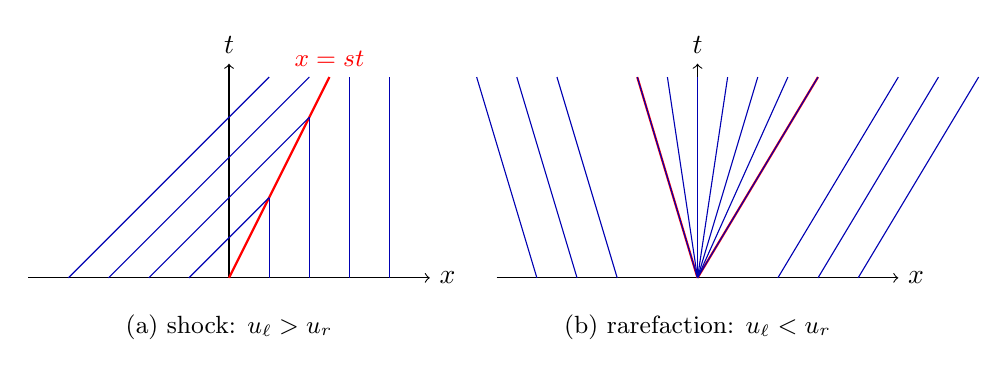
\begin{tikzpicture}[scale=0.85]
  % --- Shock case (left): u_l = 1, u_r = 0, s = 1/2 ---
  \begin{scope}
    \draw[->] (-3,0) -- (3,0) node[right] {$x$};
    \draw[->] (0,0) -- (0,3.2) node[above] {$t$};
    \draw[thick, red] (0,0) -- (1.5,3) node[above] {\small $x=st$};
    % left characteristics: speed u_l = 1, stop on hitting the shock x = t/2
    \foreach \xz in {-2.4,-1.8,-1.2,-0.6}{
      \pgfmathsetmacro{\tm}{min(3,-2*\xz)}
      \draw[blue!70!black] (\xz,0) -- ({\xz+\tm},\tm);
    }
    % right characteristics: speed u_r = 0 (vertical), stop on the shock
    \foreach \xz in {0.6,1.2,1.8,2.4}{
      \pgfmathsetmacro{\tm}{min(3,2*\xz)}
      \draw[blue!70!black] (\xz,0) -- (\xz,\tm);
    }
    \node[below] at (0,-0.4) {\small (a) shock: $u_\ell>u_r$};
  \end{scope}
  % --- Rarefaction case (right) ---
  \begin{scope}[xshift=7cm]
    \draw[->] (-3,0) -- (3,0) node[right] {$x$};
    \draw[->] (0,0) -- (0,3.2) node[above] {$t$};
    \draw[thick, red] (0,0) -- (-0.9,3);
    \draw[thick, red] (0,0) -- (1.8,3);
    \foreach \xz in {-2.4,-1.8,-1.2}{
      \draw[blue!70!black] (\xz,0) -- ({\xz-0.3*3},3);
    }
    \foreach \m in {0,1,...,6}{
      \draw[blue!70!black] (0,0) -- ({-0.9+\m*0.45},3);
    }
    \foreach \xz in {1.2,1.8,2.4}{
      \draw[blue!70!black] (\xz,0) -- ({\xz+0.6*3},3);
    }
    \node[below] at (0,-0.4) {\small (b) rarefaction: $u_\ell<u_r$};
  \end{scope}
\end{tikzpicture}
\caption{Characteristic pictures for the two cases of
Theorem~\ref{thm:riemann-solution}. (a) $u_\ell=1$, $u_r=0$, $s=1/2$:
characteristics from both sides run into the shock $x=st$. (b) Characteristics
fan out from the origin.}
\label{fig:riemann-characteristics}
\end{figure}
